\section{Methodology}

Recent developments in deep learning have greatly enhanced image-based classification tasks, notably in fine-grained domains, like textile classification. Fabric classification is uniquely complicated by the similarity of textile types (e.g., distinguishing between cotton and polyester) and variations in light and blended textile compositions. Current methods that are based on Convolutional Neural Networks (CNNs) have achieved some success with regards to fabric classification in learning local texture and patterns in fabric \cite{hong2024research, kampouris2016fine}. However, CNNs are limited in capturing long-range dependencies, or contextual information, which may be necessary for fabric classification when textiles appear similar. 

Vision Transformers (ViTs) an advanced model that can model global relationships in image data through self-attention based mechanisms \cite{dosovitskiy2020vit} have shown strong performance in generic image recognition tasks, but only few researchers have recently used it for fabric classification \cite{chitra2023fabric}. 

Driven by the pros and cons of both processes, this work proposes a hybrid deep learning model which includes CNN and ViT processes parallelly. The hybrid model leverages the \textit{local feature extraction capabilities of CNNs} and \textit{global context modeling capabilities of ViTs} to enhance classification accuracy from different textile fabric types. The proposed hybrid approach is based on the original insights from \textit{TextileNet} when the authors adopted multi-modal imaging (macro and OCT imaging) to enhance recognition of subtle structural differences found in textiles ~\cite{siam2023textilenet}.

This methodology section explains the architecture associated with this proposed model, the role played by each part of the model, details the proposed feature fusion method, and briefly covers how the final label is produced. The proposed hybrid architecture supports end-to-end training and used rigorously labeled fabric datasets to test the architecture.

\subsection{Convolutional Neural Networks (CNNs)}

Convolutional Neural Networks (CNNs) have become a cornerstone in the field of computer vision due to their effectiveness in automatically learning hierarchical feature representations from raw image data. Originally popularized for tasks such as handwritten digit recognition and object detection, CNNs have also proven highly effective in domains where texture, shape, and local patterns play a significant role—such as textile and fabric classification.

A CNN typically consists of a series of convolutional layers followed by non-linear activation functions (e.g., ReLU), pooling layers, and fully connected layers. The convolutional layers act as feature extractors, learning local filters that can detect edges, textures, and patterns at various levels of abstraction. As the network deepens, it builds increasingly complex and semantically rich representations, which are well-suited for distinguishing between different fabric types that may exhibit subtle differences in weave, fiber orientation, or surface reflectivity~\cite{simonyan2015vgg, lecun1998gradient}.

In this work, a CNN-based stream is designed as part of a hybrid model, consisting of four convolutional blocks with progressively increasing output channels (8, 16, 32, 64). Each block applies a $3\times3$ convolution operation with a stride of 3, followed by a ReLU activation. This architecture efficiently reduces the spatial resolution while preserving essential texture and pattern information—a technique previously shown to be effective in textile classification tasks~\cite{hong2024research}.

Studies such as by Kampouris et al.~\cite{kampouris2016fine} and Hong et al.~\cite{hong2024research} have demonstrated the success of CNNs in classifying fabric materials based on surface and structural characteristics. Furthermore, in practical applications, CNNs have been favored for their ability to generalize well to real-world textile images, including those captured under varying lighting conditions and camera settings.

While CNNs are powerful in learning local features, they are inherently limited in capturing global dependencies across spatial regions, which may affect performance when dealing with patterned fabrics. To address this limitation, CNNs are combined in this study with Vision Transformer (ViT) encoders, described in the following section, to capture both local and global representations of fabric structures.

\subsection{Vision Transformers (ViTs)}

Vision Transformers (ViTs) have emerged as a powerful alternative to convolutional architectures for image classification tasks. Unlike Convolutional Neural Networks (CNNs), which operate on local receptive fields, ViTs leverage self-attention mechanisms to model global relationships between different parts of an image. This makes them particularly suitable for applications like fabric classification, where understanding the spatial layout and contextual relationships between texture patterns is important~\cite{dosovitskiy2020vit}.

A standard Vision Transformer operates by first dividing an image into fixed-size patches (e.g., $16 \times 16$ pixels), which are flattened and projected into a latent embedding space using a linear layer. These patch embeddings, along with a learnable class token and positional encodings, are passed into a stack of Transformer encoder layers. Each encoder layer consists of two main subcomponents:
\begin{itemize}
    \item \textbf{Multi-Head Self-Attention (MHSA):} Computes pairwise attention scores between patches, enabling the model to capture long-range dependencies.
    \item \textbf{Feed-Forward Network (FFN):} A two-layer fully connected network with non-linearity (typically GELU), applied independently to each patch embedding.
\end{itemize}

Layer normalization and residual connections are applied around both subcomponents to enhance training stability. The final output corresponding to the class token is used for classification purposes.

In this study, the ViT branch consists of four sequential Transformer encoder layers, each of which processes the patch embeddings generated from the input image. The aim is to extract \textit{global and contextual features} that are particularly useful when dealing with fabrics that contain repeating patterns, folds, or blended fibers, where large-scale spatial context contributes to accurate classification~\cite{chitra2023fabric, siam2023textilenet}.

While CNNs are inherently biased toward local feature extraction, ViTs offer greater flexibility by modeling relationships across the entire image without positional locality assumptions. This property makes them highly effective in fabric classification scenarios, where a fiber's spatial structure can influence its identification. Moreover, recent research shows that ViTs can outperform CNNs when trained on sufficiently large datasets or when used in hybrid systems~\cite{dosovitskiy2020vit, touvron2021training}.

By integrating a ViT stream in parallel with a CNN stream, this work aims to build a hybrid system capable of leveraging both local textures and global structure, resulting in a more robust and accurate fabric classification model.

\subsection{Feature Fusion and Classification}

Once the image has been processed independently by the Convolutional Neural Network (CNN) and Vision Transformer (ViT) branches, the resulting feature maps from both streams are merged to form a unified representation. This step is critical, as it combines the advantages of both local texture sensitivity (from CNN) and global contextual awareness (from ViT), enabling the model to make more informed predictions.

\paragraph{Feature Stacking}

The output of the final convolutional layer in the CNN stream and the final encoder layer in the ViT stream are first flattened and then concatenated along the feature dimension. This operation creates a stacked feature vector of dimension 1024, which encapsulates the most informative characteristics extracted from both branches. Feature-level fusion techniques such as concatenation are commonly used in multi-stream architectures to preserve complementary representations before classification~\cite{zhong2023textilenet, chitra2023fabric, xu2018multichannel}.

\begin{figure}[ht]
    \centering
    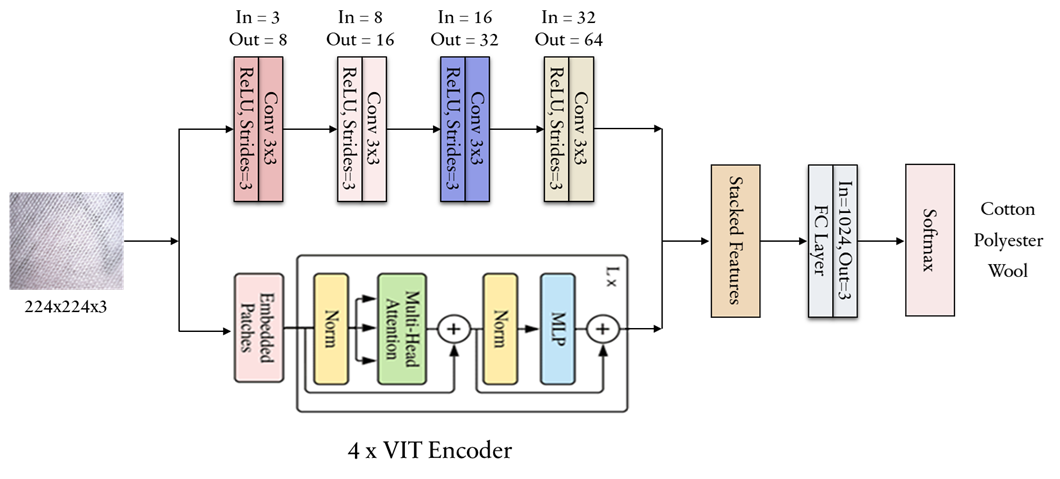
\includegraphics[width=0.95\textwidth]{images/ModelDiagram.png}
    \caption{The proposed hybrid CNN–ViT architecture for fabric classification.}
    \label{fig:model-architecture}
\end{figure}

\paragraph{Fully Connected Layer}

The stacked feature vector is passed through a fully connected (FC) layer, which serves as the final transformation before classification. The FC layer acts as a dense classifier that maps the high-dimensional feature space into a 3-dimensional output, each corresponding to one of the fabric classes.

Mathematically, the output logits \( z \in \mathbb{R}^3 \) are computed as:
\[
z = W_f x + b_f
\]
where:
\begin{itemize}[noitemsep,topsep=0pt]
    \item \( x \in \mathbb{R}^{1024} \) is the input stacked feature vector,
    \item \( W_f \in \mathbb{R}^{3 \times 1024} \) is the weight matrix of the FC layer,
    \item \( b_f \in \mathbb{R}^{3} \) is the bias term.
\end{itemize}

\paragraph{Softmax Classification}

To obtain the final prediction, the output logits are passed through the Softmax activation function, which converts the raw scores into a probability distribution over the three fabric classes:

\[
\text{Softmax}(z_i) = \frac{e^{z_i}}{\sum_{j=1}^{3} e^{z_j}}, \quad \text{for } i = 1,2,3
\]

This ensures that the output probabilities are non-negative and sum to 1. The class with the highest probability is selected as the final predicted label. The use of softmax is standard in multi-class classification tasks and is particularly effective when combined with cross-entropy loss during training~\cite{bishop2006pattern, goodfellow2016deep}.